\clearpage
\section{Realisierung Gehäuse}\label{sec:Realisierung Gehäuse}
Im folgenden Teil des Fachberichtes ist die Realisierung des Gehäuses beschrieben. 

Die Anforderungen an das Gehäuse des digitalen Theremins sind:
\begin{itemize}
	\item Die Lautstärken- und die Tonhöhenantenne müssen genügend Abstand zueinander haben, damit der Spieler das Theremin richtig spielen kann.
	\item Das Antennenoszillator PCB und das DE1-SoC Board müssen für den Spieler ersichtlich sein.
	\item Für die Bedienung muss das LT24 Touch Modul für den Benutzer gut sichtbar platziert sein.
	\item Um den Preis des Gehäuses tief zu halten und für die Gestaltung des Gehäuses möglichst viel Freiheit zu haben, soll das Gehäuse 3D-gedruckt sein.  
\end{itemize}

Um diese Anforderungen zu erfüllen, konstruierten wir das Gehäuse mit dem 3D-CAD-System Inventor. Inventor ist eine sehr umfangreiche Konstruktions-Software mit dem die ausgefallene Form des Gehäuses leicht zu realisieren war.
Um das Gehäuse zu drucken, verwendeten wir den S5 Ultimaker 3D Drucker, da dieser sehr benutzerfreundlich ist und ein grosses Druckvolumen hat. 
Der S5 Drucker hat ein Druckvolumen von \SI{330x240x300}{mm}. 
Das Gehäuse musste jedoch in vier Teile unterteilt werden, damit die Platzverhältnisse im Drucker ausreichten. 

Wir gestalteten die Form des Theremins oval, da andere kommerziell erhältliche Theremins eine solche Form aufweisen. Die vier Einzelteile des Gehäuses sind alle gleich aufgebaut. Abbildung \ref{img:grundteil} zeigt die Grundstruktur eines Einzelteils. Die Funktion Wandung von Inventor ermöglichte es, die Grundstruktur oval auszuhöhlen. Jeweils zwei Einzelteile bilden zusammen den Deckel und den Boden. Daraus resultierte das in Abbildung \ref{img:Theremin_case} gezeigte Gehäuse. 

Die vier Einzelteile bestehen aus schwarzem Polylactide (PLA). Da das Gehäuse eine ovale Geometrie hat, braucht es Stützstrukturen für den Herstellungsprozess. Das eingesetzte Polyvinylalkohol (PVAL) hat die nützliche Eigenschaft, das es wasserlösslich ist.
\begin{figure}[h]
	\centering
	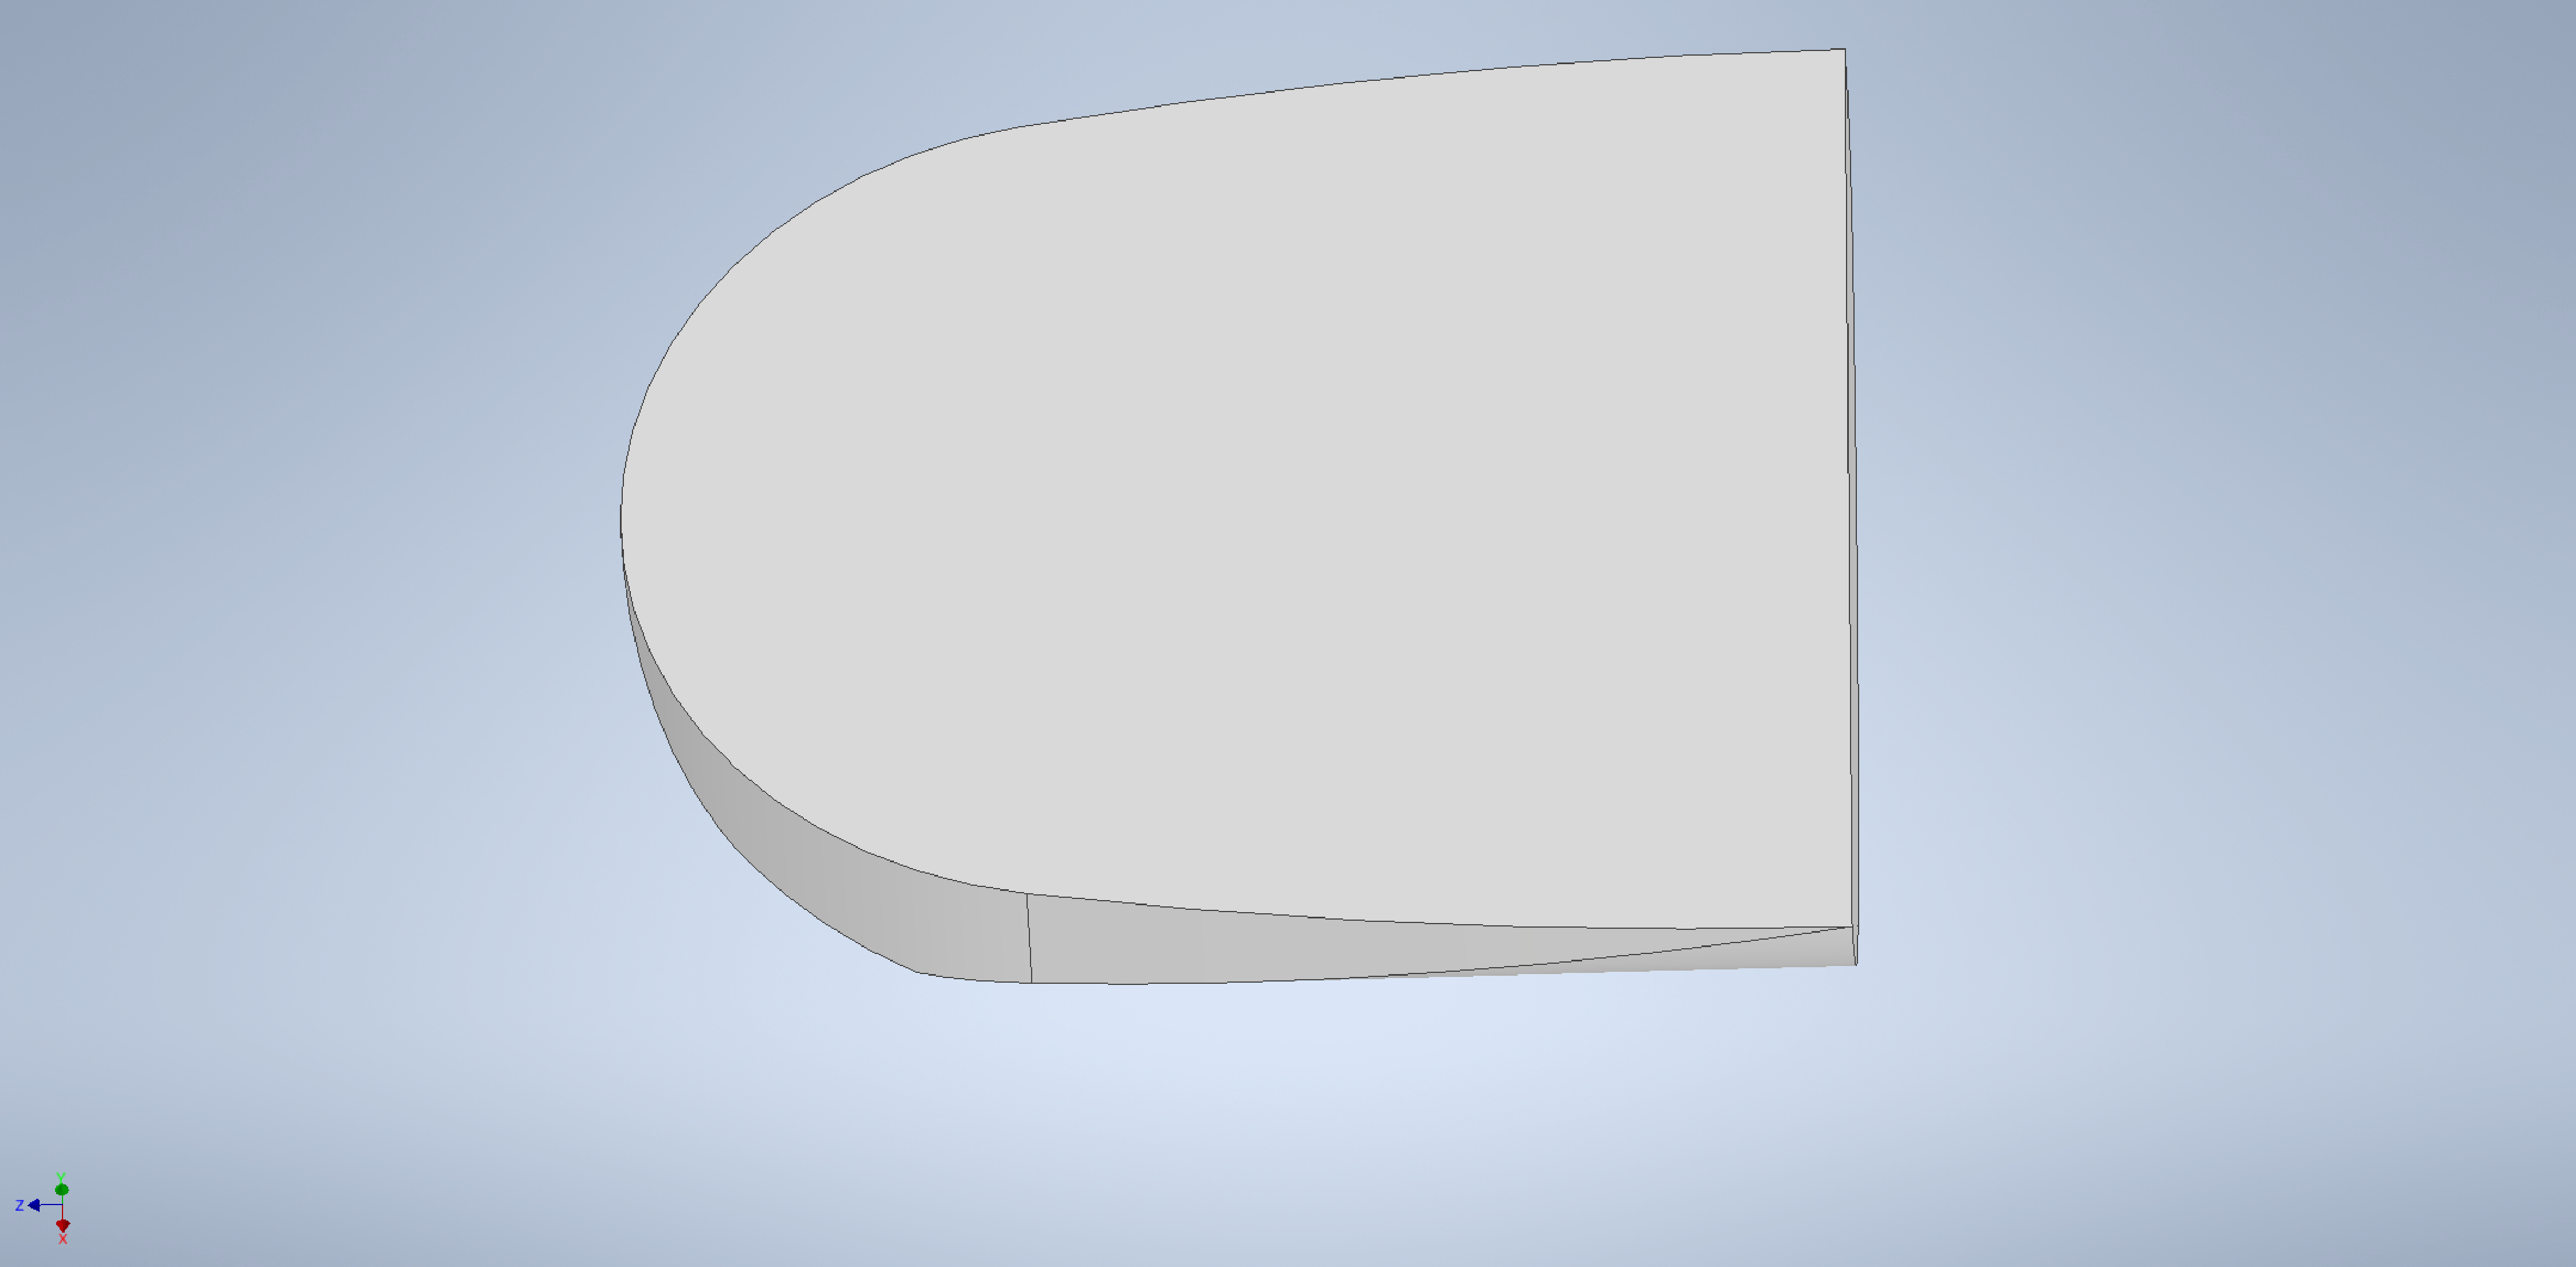
\includegraphics[width=\textwidth]{grundteil.pdf}
	\caption{Grundstruktur eines Einzelteils.}
	\label{img:grundteil}
\end{figure}
\begin{figure}[h]
	\centering
	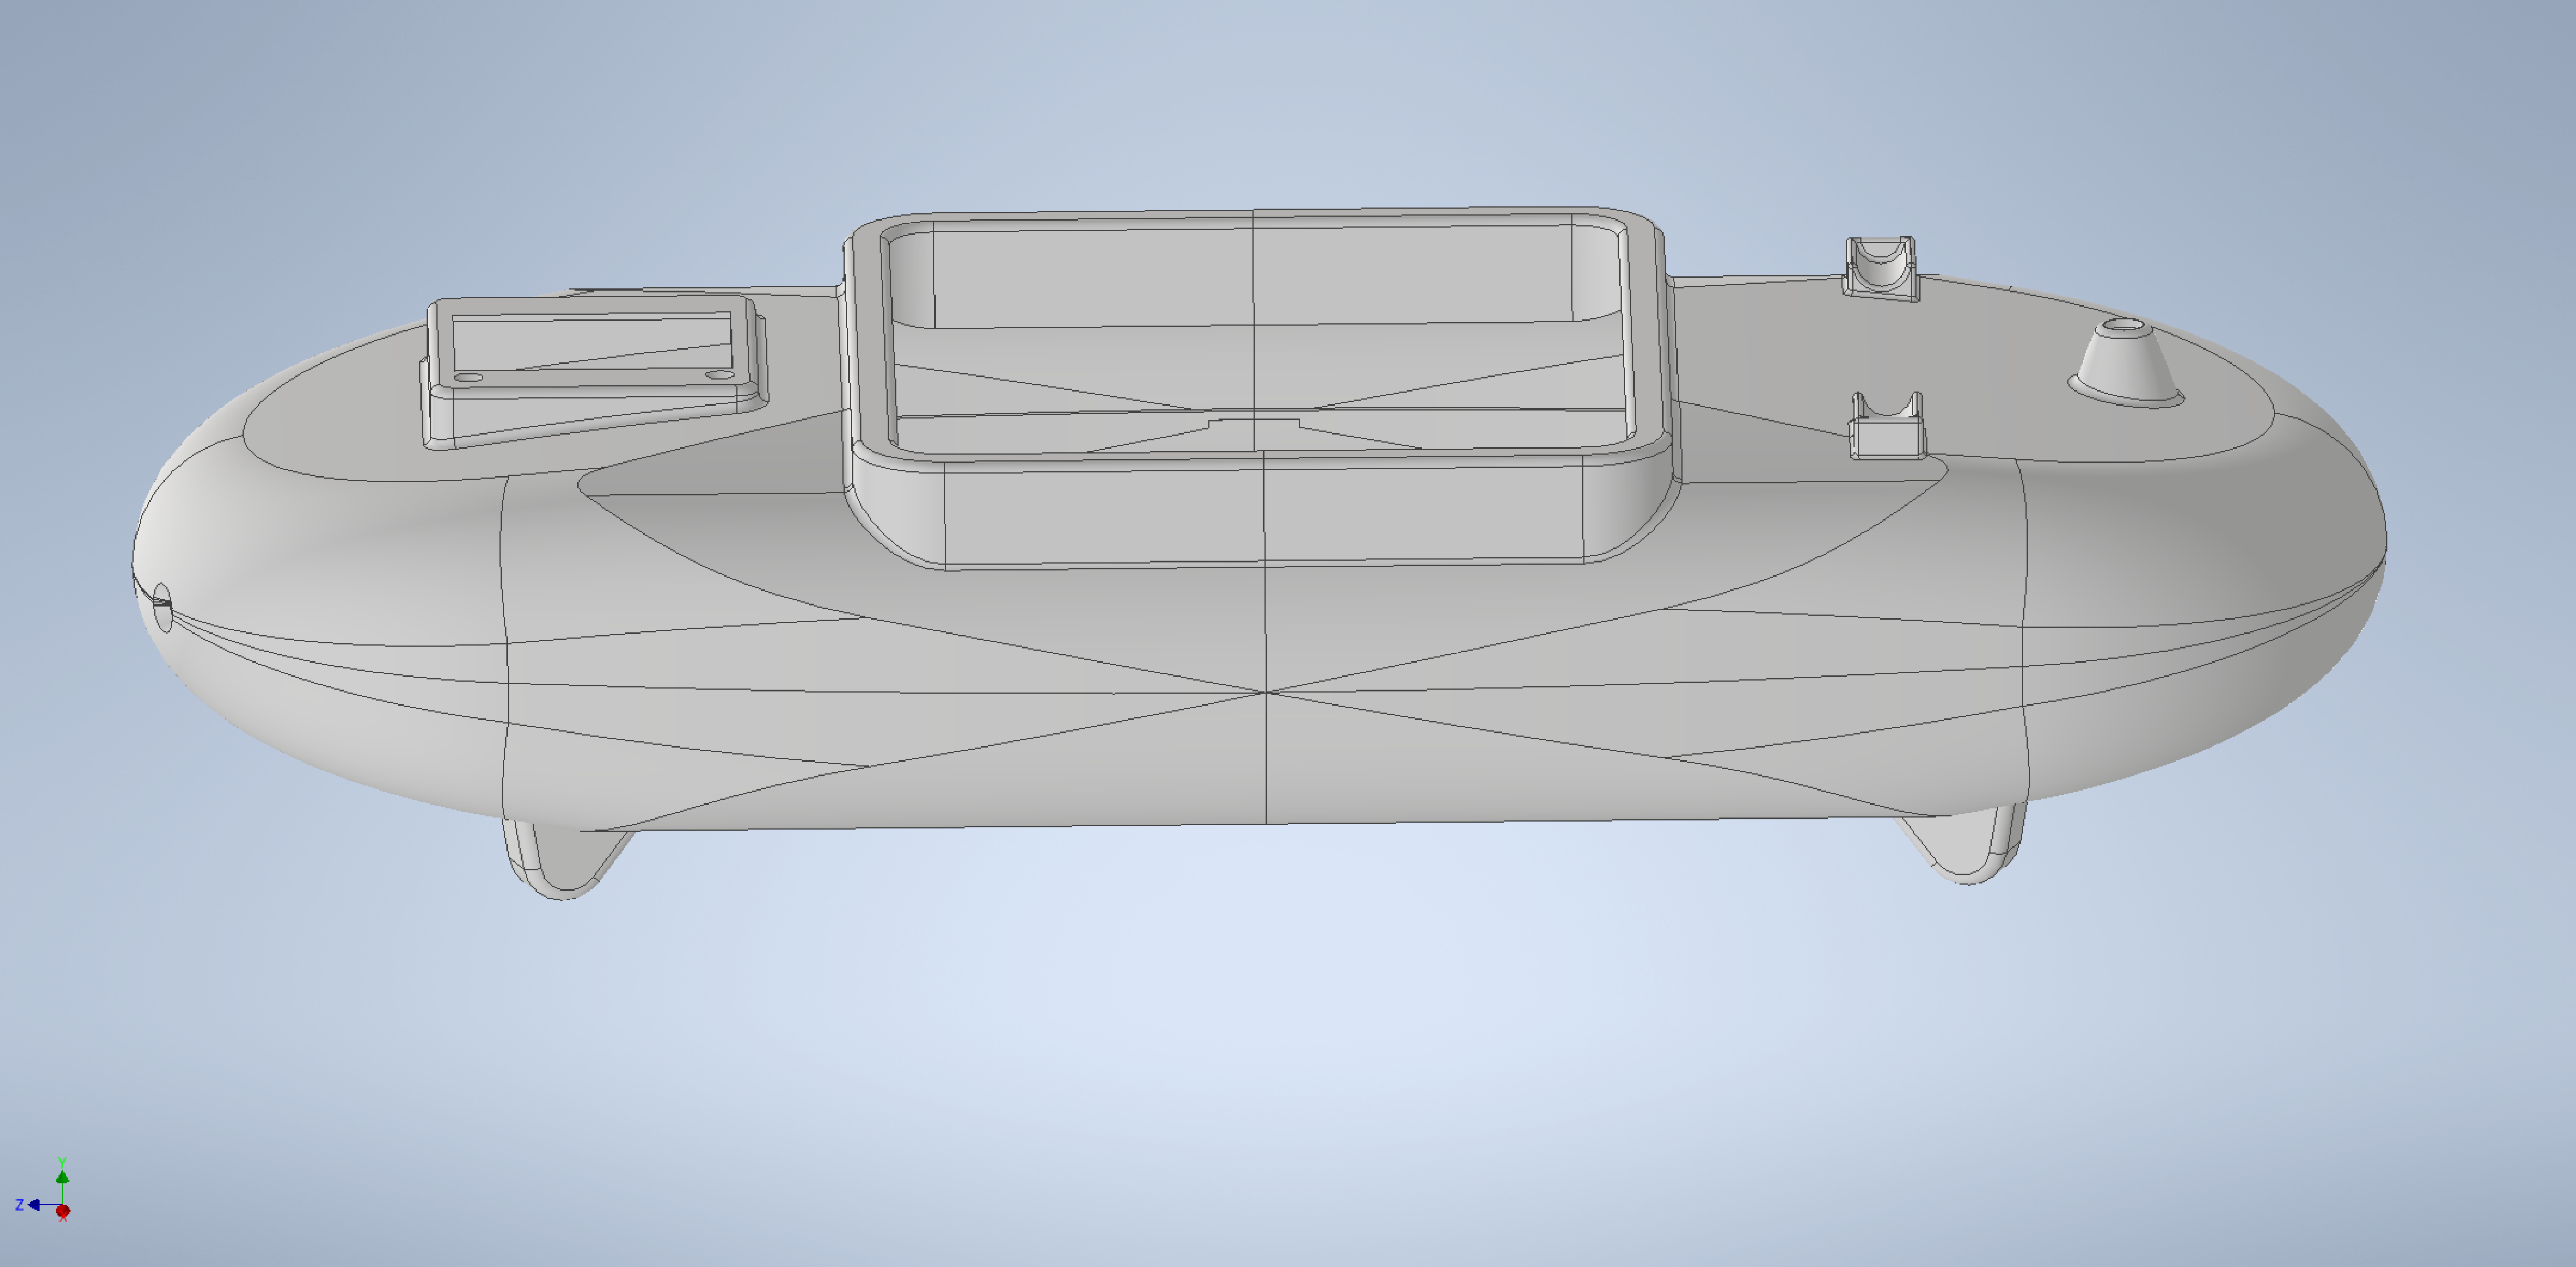
\includegraphics[width=\textwidth]{Theremin_case.pdf}
	\caption{Theremin-Gehäuse.}
	\label{img:Theremin_case}
\end{figure}
\begin{figure}[h]
	\centering
	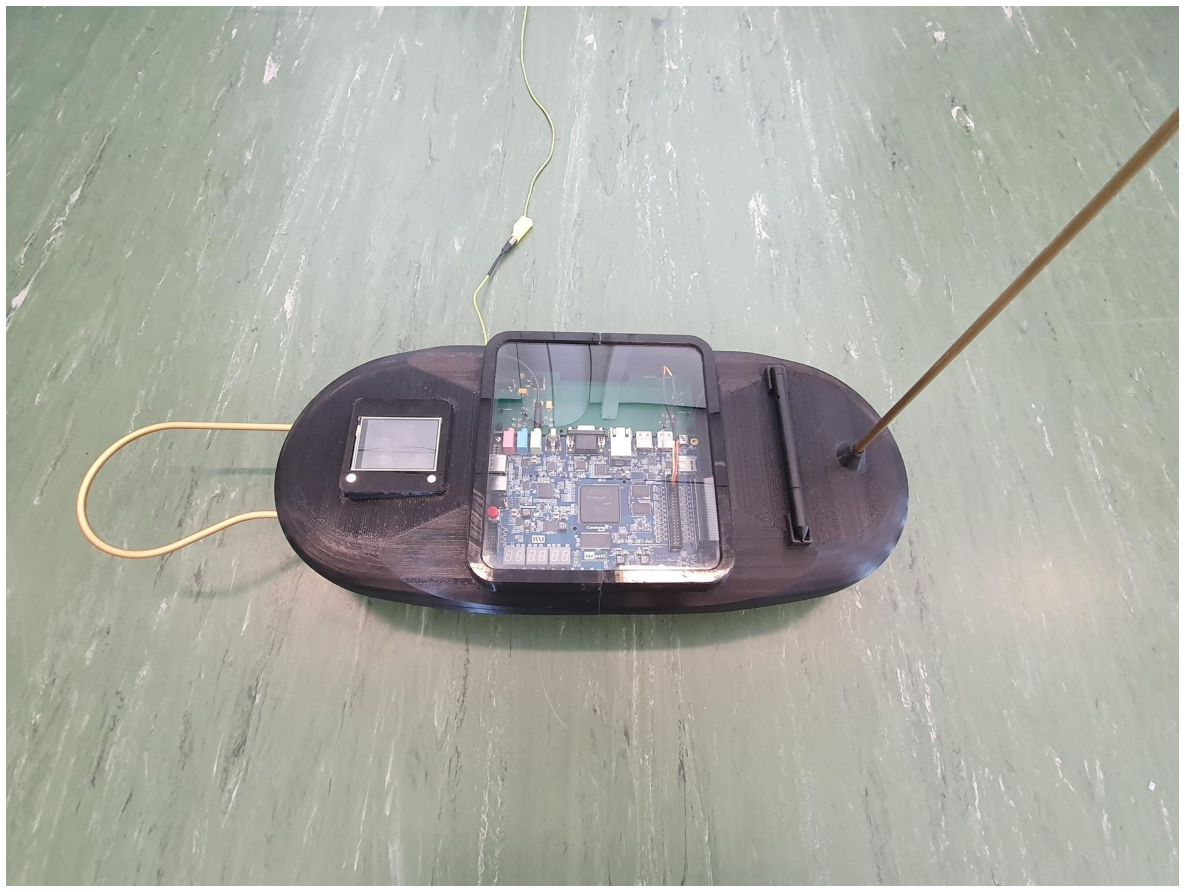
\includegraphics[width=\textwidth]{Theremin_komplett.pdf}
	\caption{kompletter Aufbau des Theremins}
	\label{img:Theremin_komplett}
\end{figure}




